% Copyright 2011-2014 David Hadka.  All Rights Reserved.
%
% This file is part of the MOEA Framework User Manual.
%
% Permission is granted to copy, distribute and/or modify this document under
% the terms of the GNU Free Documentation License, Version 1.3 or any later
% version published by the Free Software Foundation; with the Invariant Section
% being the section entitled "Preface", no Front-Cover Texts, and no Back-Cover
% Texts.  A copy of the license is included in the section entitled "GNU Free
% Documentation License".

\chapter{Introduction}

The MOEA Framework is a free and open source Java library for developing and experimenting with multiobjective evolutionary algorithms (MOEAs) and other general-purpose optimization algorithms.  A number of algorithms are provided out-of-the-box, including NSGA-II, $\epsilon$-MOEA, GDE3 and MOEA/D.  In addition, the MOEA Framework provides the tools necessary to rapidly design, develop, execute and statistically test optimization algorithms.

This user manual is divided into the following three parts:
\begin{description}
  \item [Beginner's Guide] - Provides an introduction to the MOEA Framework for new users.  Topics discussed include installation instructions, walking through some introductory examples, and solving user-specified problems.
  \item [Advanced Guide] - Introduces features provided by the MOEA Framework intended for academic researchers and other advanced users.  Topics include performing large-scale experimentation, statistically comparing algorithms, and advanced configuration options.
  \item [Developer's Guide] - Intended for software developers, this part details guidelines for contributing to the MOEA Framework.  Topics covered include the development of new optimization algorithms, software coding guidelines and other policies for contributors.
\end{description}

\begin{important}
Throughout this manual, you will find paragraphs marked with a red exclamation as shown on the left-hand side of this page.  This symbol indicates important advice to help troubleshoot common problems.
\end{important}

\begin{tip}
Additionally, paragraphs marked with the lightbulb, as shown to the left, provide helpful suggestions and other advice.  For example, here is perhaps the best advice we can provide: throughout this manual, we will refer you to the ``API documentation'' to find additional information about a feature.  The API documentation is available at \webpage{http://moeaframework.org/javadoc/index.html}.  This documentation covers every aspect and every feature of the MOEA Framework in detail, and it is the best place to look to find out how something works.
\end{tip}

\section{Key Features}

The following features of the MOEA Framework distinguish it from available alternatives (detailed in the next section).

\paragraph{Fast, reliable implementations of many state-of-the-art multiobjective evolutionary algorithms.}  The MOEA Framework contains internally NSGA-II, $\epsilon$-MOEA, $\epsilon$-NSGA-II, GDE3 and MOEA/D.  These algorithms are optimized for performance, making them readily available for high performance applications.  By also supporting the JMetal and PISA libraries, the MOEA Framework provides access to $24$ multiobjective optimization algorithms.

\paragraph{Extensible with custom algorithms, problems and operators.}  The MOEA Framework provides a base set of algorithms, test problems and search operators, but can also be easily extended to include additional components.  Using a Service Provider Interface (SPI), new algorithms and problems are seamlessly integrated within the MOEA Framework.  

\paragraph{Modular design for constructing new optimization algorithms from existing components.}  The well-structured, object-oriented design of the MOEA Framework library allows combining existing components to construct new optimization algorithms.  And if needed functionality is not available in the MOEA Framework, you can always extend an existing class or add new classes to support any desired feature.

\paragraph{Permissive open source license.}  The MOEA Framework is licensed under the free and open GNU Lesser General Public License, version 3 or (at your option) any later version.  This allows end users to study, modify, and distribute the MOEA Framework freely.

\paragraph{Fully documented source code.}  The source code is fully documented and is frequently updated to remain consistent with any changes.  Furthermore, an extensive user manual is provided detailing the use of the MOEA Framework in detail.

\paragraph{Extensive support available online.}  As an actively maintained project, bug fixes and new features are constantly added.  We are constantly striving to improve this product.  To aid this process, our website provides the tools to report bugs, request new features, or get answers to your questions.

\paragraph{Over 1100 test cases to ensure validity.}  Every release of the MOEA Framework undergoes extensive testing and quality control checks.  And, if any bugs are discovered that survive this testing, we will promptly fix the issues and release patches.  

\section{Other Java Frameworks}
There exist a number of Java optimization framework developed over the years.  This section discusses the advantages and disadvantages of each framework.  While we appreciate your interest in the MOEA Framework, it is always useful to be aware of the available tools which may suit your specific needs better.

\subsection{Watchmaker Framework}
\begin{wrapfigure}{l}{4cm}
  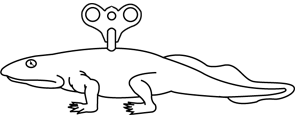
\includegraphics[width=4cm]{watchmaker.png}
\end{wrapfigure}
The Watchmaker Framework is one of the most popular open source Java libraries for single objective optimization.  Its design is non-invasive, allowing users to evolve objects of any type.  Most other frameworks (including the MOEA Framework) require the user to encode their objects using pre-defined decision variable types.  However, giving the users this freedom also increases the burden on the user to develop custom evolutionary operators for their objects.

\begin{quote}
\begin{description}
  \item[Homepage:] \webpage{http://watchmaker.uncommons.org}
  \item[License:] Apache License, Version 2.0
  \item[Advantages:]\ %force line break
    \begin{itemize}
      \item Very clean API
      \item Fully documented source code
      \item Flexible decision variable representation
      \item Large collection of interesting example problems (Mona Lisa, Sudoku, Biomorphs)
    \end{itemize}
  \item[Disadvantages:]\ %force line break
    \begin{itemize}
      \item Single objective only
      \item Much of the implementation burden is placed on the developer
      \item Infrequently updated (the last release, 0.7.1, was in January 2010)
    \end{itemize}
\end{description}
\end{quote}

\subsection{ECJ}
ECJ is a research-oriented Java library developed at the George Mason University's Evolutionary Computation Laboratory.  Now in existence for nearly fourteen years, ECJ is a mature and stable framework.  It features a range of evolutionary paradigms, including both single and multiobjective optimization, master/slave and island-model parallelization, coevolution, parsimony pressure techniques, with extensive support for genetic programming.  

\begin{quote}
\begin{description}
  \item[Homepage:] \webpage{http://cs.gmu.edu/~eclab/projects/ecj/}
  \item[License:] Academic Free License, Version 3.0
  \item[Advantages:]\ %force line break
    \begin{itemize}
      \item Quickly setup and execute simple EAs without touching any source code
      \item One of the most sophisticated open source libraries, particular in its support for various GP tree encodings
      \item Provides an extensive user manual, tutorials, and other developer tools
    \end{itemize}
  \item[Disadvantages:]\ %force line break
    \begin{itemize}
      \item Focused on single-objective optimization, providing only older MOEAs (NSGA-II and SPEA2)
      \item Configuring EAs using ECJ�s configuration file can be cumbersome and error prone
      \item Appears to lack any kind of automated testing or quality assurance
    \end{itemize}
\end{description}
\end{quote}

\subsection{jMetal}
jMetal \index{jMetal} is a framework focused on the development, experimentation and study of metaheuristics.  As such, it includes the largest collection of metaheuristics of any framework discussed here.  If fact, the MOEA Framework incorporates the jMetal library for this very reason.  The jMetal authors have more recently started developing C++ and C\# versions of the jMetal library. 

\begin{quote}
\begin{description}
  \item[Homepage:] \webpage{http://jmetal.sourceforge.net}
  \item[License:] GNU Lesser General Public License, Version 3 or later
  \item[Advantages:]\ %force line break
    \begin{itemize}
      \item Focused on multiobjective optimization
      \item Implementations of 15 state-of-the-art MOEAs
      \item Provides an extensive user manual
    \end{itemize}
  \item[Disadvantages:]\ %force line break
    \begin{itemize}
      \item Not currently setup as a library; several places have hard-coded paths to resources located on the original developer�s computer
      \item Appears to lack any kind of automated testing or quality assurance
      \item Source code is not fully documented
    \end{itemize}
\end{description}
\end{quote}

\subsection{Opt4J}
\begin{wrapfigure}{l}{4cm}
  
\includegraphics[width=4cm]{opt4j.png}
\end{wrapfigure}
Opt4J provides perhaps the cleanest MOEA implementation.  It takes modularity to the extreme, using aspect-oriented programming to automatically stitch together program modules to form a complete, working optimization algorithm.  A helpful GUI for constructing experiments is also provided.

\begin{quote}
\begin{description}
  \item[Homepage:] \webpage{http://opt4j.sourceforge.net/}
  \item[License:] GNU Lesser General Public License, Version 3 or later
  \item[Advantages:]\ %force line break
    \begin{itemize}
      \item Focused on multiobjective optimization
      \item Uses aspect-oriented programming (AOP) via Google Guice to manage dependencies and wire all the components together
      \item Well documented source code
      \item Frequently updated
    \end{itemize}
  \item[Disadvantages:]\ %force line break
    \begin{itemize}
      \item Only a limited number of MOEAs provided
    \end{itemize}
\end{description}
\end{quote}

\subsection{Others}
For completeness, we also acknowledge JGAP and JCLEC, two stable and maintained Java libraries for evolutionary computation.  These two libraries, like the Watchmaker Framework, are specialized for single-objective optimization.  They do provide basic support for multiobjective optimization, but not to the extent of JMetal, Opt4J, and the MOEA Framework.  If you are dealing with only single-objective optimization problems, we encourage you to explore these libraries that specialize in single-objective optimization.

\section{Reporting Bugs}
The MOEA Framework is not bug-free, nor is any other software application, and reporting bugs to developers is the first step towards improving the reliability of software.  Critical bugs will often be addressed within days.  If during its use you encounter error messages, crashes, or other unexpected behavior, please file a bug report at \webpage{http://moeaframework.org/support.html}.  In the bug report, describe the problem encountered and, if known, the version of the MOEA Framework used.

\section{Getting Help}
This user guide is the most comprehensive resource for learning about the MOEA Framework.  However, as this manual is still a work in progress, you may need to turn to some other resources to find answers to your questions.  Our website at \webpage{http://www.moeaframework.org} contains links to the API documentation, which provides access to the detailed source code documentation.  This website also has links to file bugs or request new features.  If you still can not find an answer to your question, feel free to contact us at \mailto{support@moeaframework.org}.